\section{Results}
\label{sec:results}

The experiments were performed on the Frontier~\cite{frontier} supercomputer at Oak Ridge National Laboratory.
%Summit is a 200 PetaFLOPS supercomputer that consists of 4608 nodes. Each node contains two 22-core IBM Power9 CPUs and six NVIDIA Tesla V100 GPUs.
Frontier is a 1.102 ExaFLOPS supercomputer consisting of 9472 nodes. Each node contains a 64-core AMD Epyc CPU and four Radeon Instinct MI250X GPUs. 


\begin{comment}
\begin{figure}[ht]
 \centering
  \subfigure[Whole seeding]{
    \label{fig:seedingUniform}  
     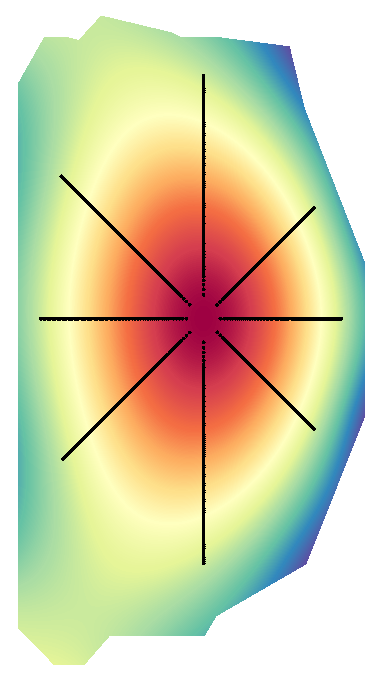
\includegraphics[width=25mm]{figures/seedingWhole}
   }
  \subfigure[Edge seeding]{
   \label{fig:seedingEdge}  
   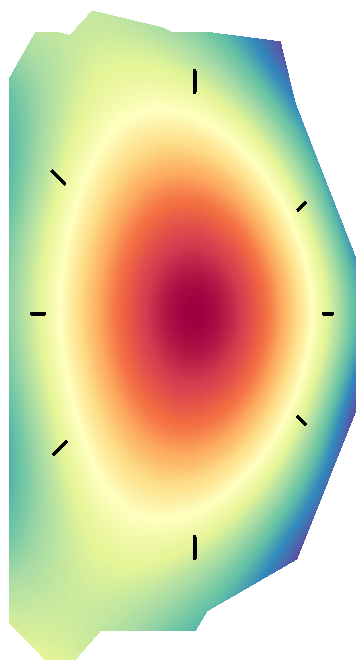
\includegraphics[width=25mm]{figures/seedingEdge}
   }

\caption{Seed placement provides opportunities for analysis of different parts of the plasma. Whole seeding (a), provides an overall view of the magnetic field. Edge seeding (b), is useful to analyze the outer region of the plasma where turbulence is very high. }
\vspace{-5pt}
\label{fig:seeding}
\end{figure}
\end{comment}


\begin{figure}[ht]
 \centering
  \subfigure[Whole seeding]{
    \label{fig:seedingUniform}  
     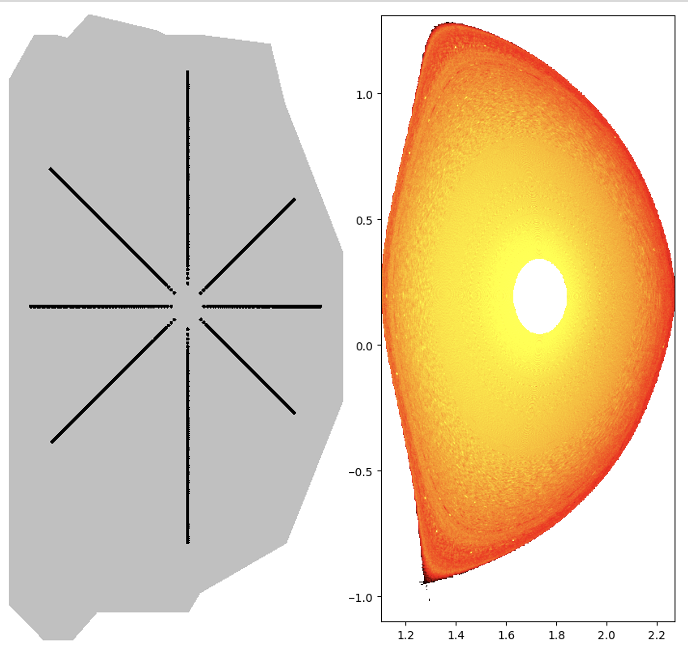
\includegraphics[height=30mm]{figures/wholeSeedingAndResult}
   }
  \subfigure[Edge seeding]{
   \label{fig:seedingEdge}  
   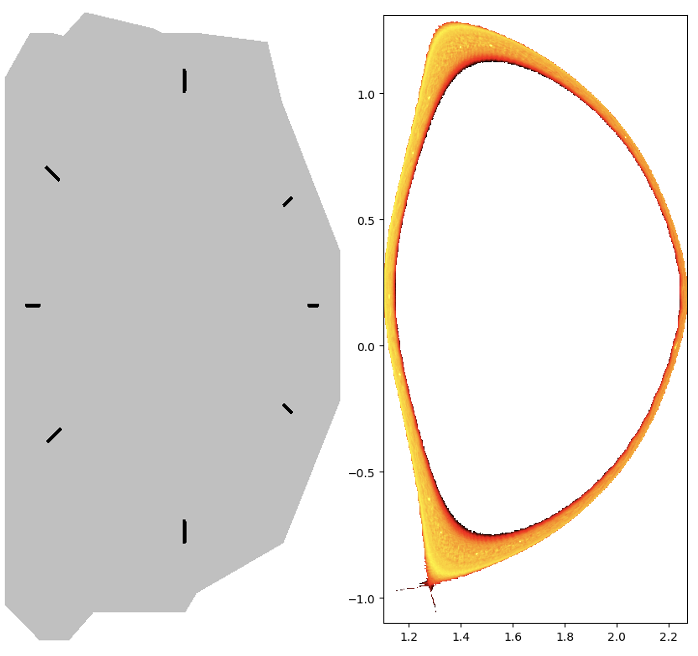
\includegraphics[height=30mm]{figures/edgeSeedingAndResult}
   }

\caption{Seed placement allows for analysis of different parts of the plasma. Whole seeding along with the resulting \poincare map is shown in (a), and the edge seeding and results are shown in (b).}
\vspace{-5pt}
\label{fig:seeding}
\end{figure}


To study the performance, we ran both the XGC and \vtkm versions of the \poincare tool. We use the XGC implementation as a baseline. While the XGC simulation code can run on GPUs, the XGC \poincare\ analysis tool is only implemented on the CPUs. 
The \vtkm implementation was run on both the CPU and GPU. The results from the runs on CPUs give us a direct comparison between the XGC analysis code and the \vtkm equivalent. The runs on the GPU highlight the added benefits afforded by the portability of the \vtkm implementation.

The XGC implementation was run on the CPUs of five Frontier nodes and uses OpenMP for parallelization across the multi-core CPUs.
The \vtkm implementation was run in two configurations -- CPU and GPU.
The CPU implementation was run on two Frontier nodes and the GPU implementation was run on a single node using two of the four GPUs.

We used two variations in the number of seeds and two variations in the placement of the seeds for a total of four different configurations.
The seeds are placed along regular angular intervals around the center of the cross-section. We used a total of eight angular intervals and placed $1280$ and $3200$ seeds along each angular interval. This gives seed numbers of 10,240 and 25,600. We also varied the placement of the seeds along each angular interval. For whole seeding (see Figure~\ref{fig:seedingUniform}), the seeds are placed uniformly from the center of the cross-section to the edge. For edge seeding (see Figure~\ref{fig:seedingEdge}), the seeds are placed further away from the center, or nearer to the edge of the plasma.  Whole seed placement is used to analyze the overall nature of the magnetic field in the plasma. The placement of seeds along the edge is a common way to analyze the very turbulent regions of the plasma that occur along the edge region. Figure~\ref{fig:result} shows a zoomed-in view of \poincare maps generated from two different time steps using edge seeding. The image is zoomed in to view the bottom left of the cross-section, called the ''X'' point, where turbulence in the plasma is complex.


\begin{comment}
\begin{figure}[ht]
 \centering
  \subfigure[Whole seeding. ]{
    \label{fig:resultUniform}  
     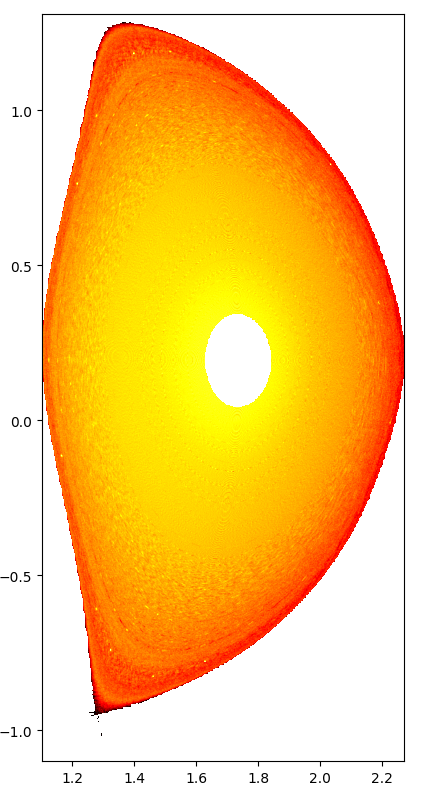
\includegraphics[width=20mm]{figures/whole}
     }
  \subfigure[Edge seeding.]{
   \label{fig:resultEdge}  
   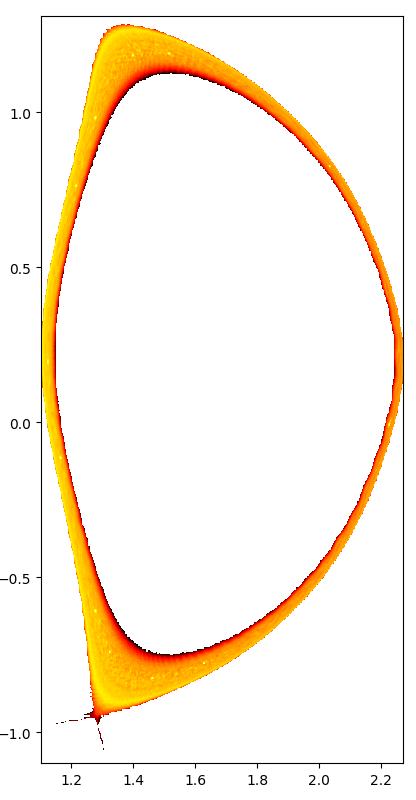
\includegraphics[width=20mm]{figures/edge}
   }

\caption{Resulting \poincare plots from 10,240 seeds using whole (a) and edge (b) seeding.}
\vspace{-5pt}
\label{fig:result}
\end{figure}
\end{comment}


\begin{figure}[ht]
 \centering
 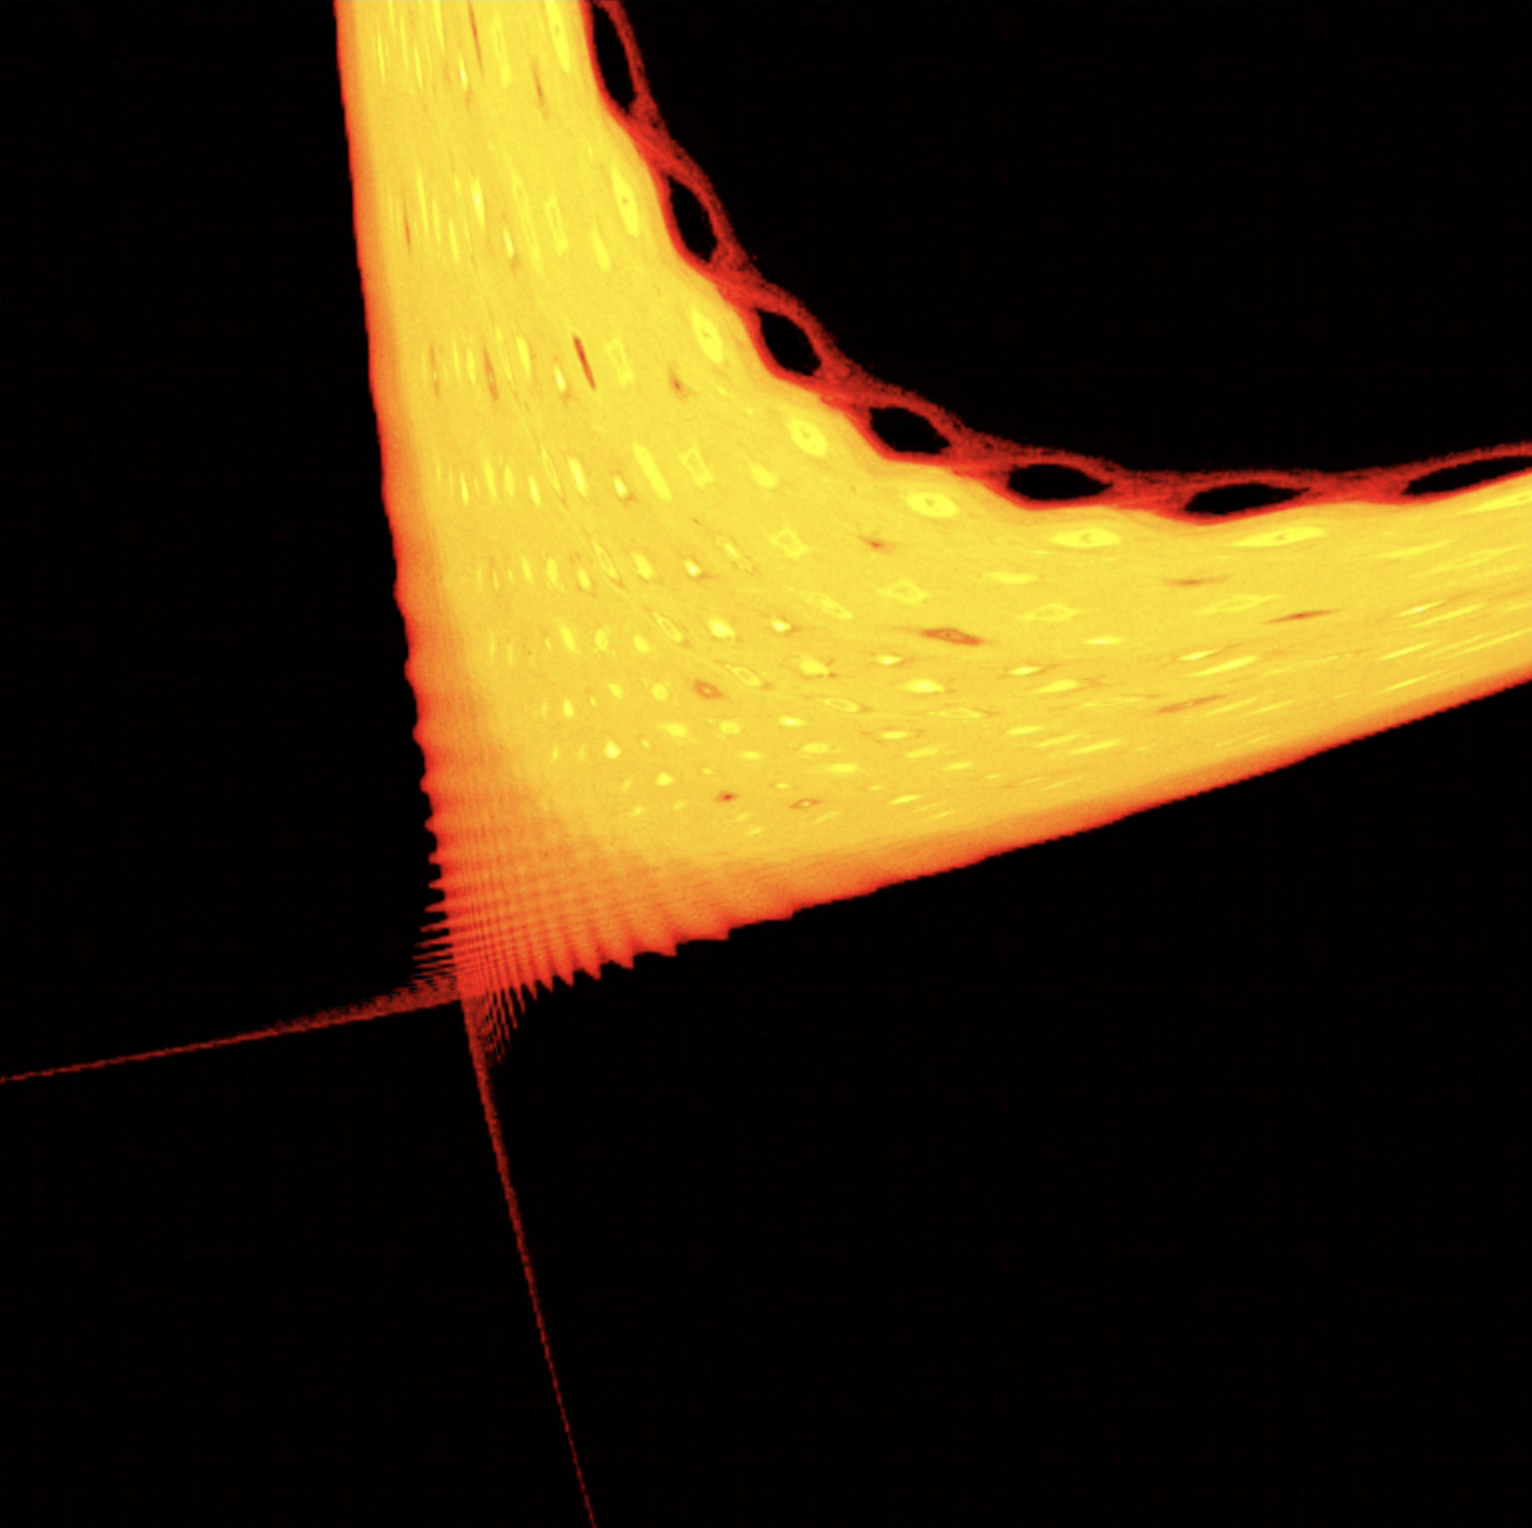
\includegraphics[width=40mm]{figures/poincare-X.1.png}
 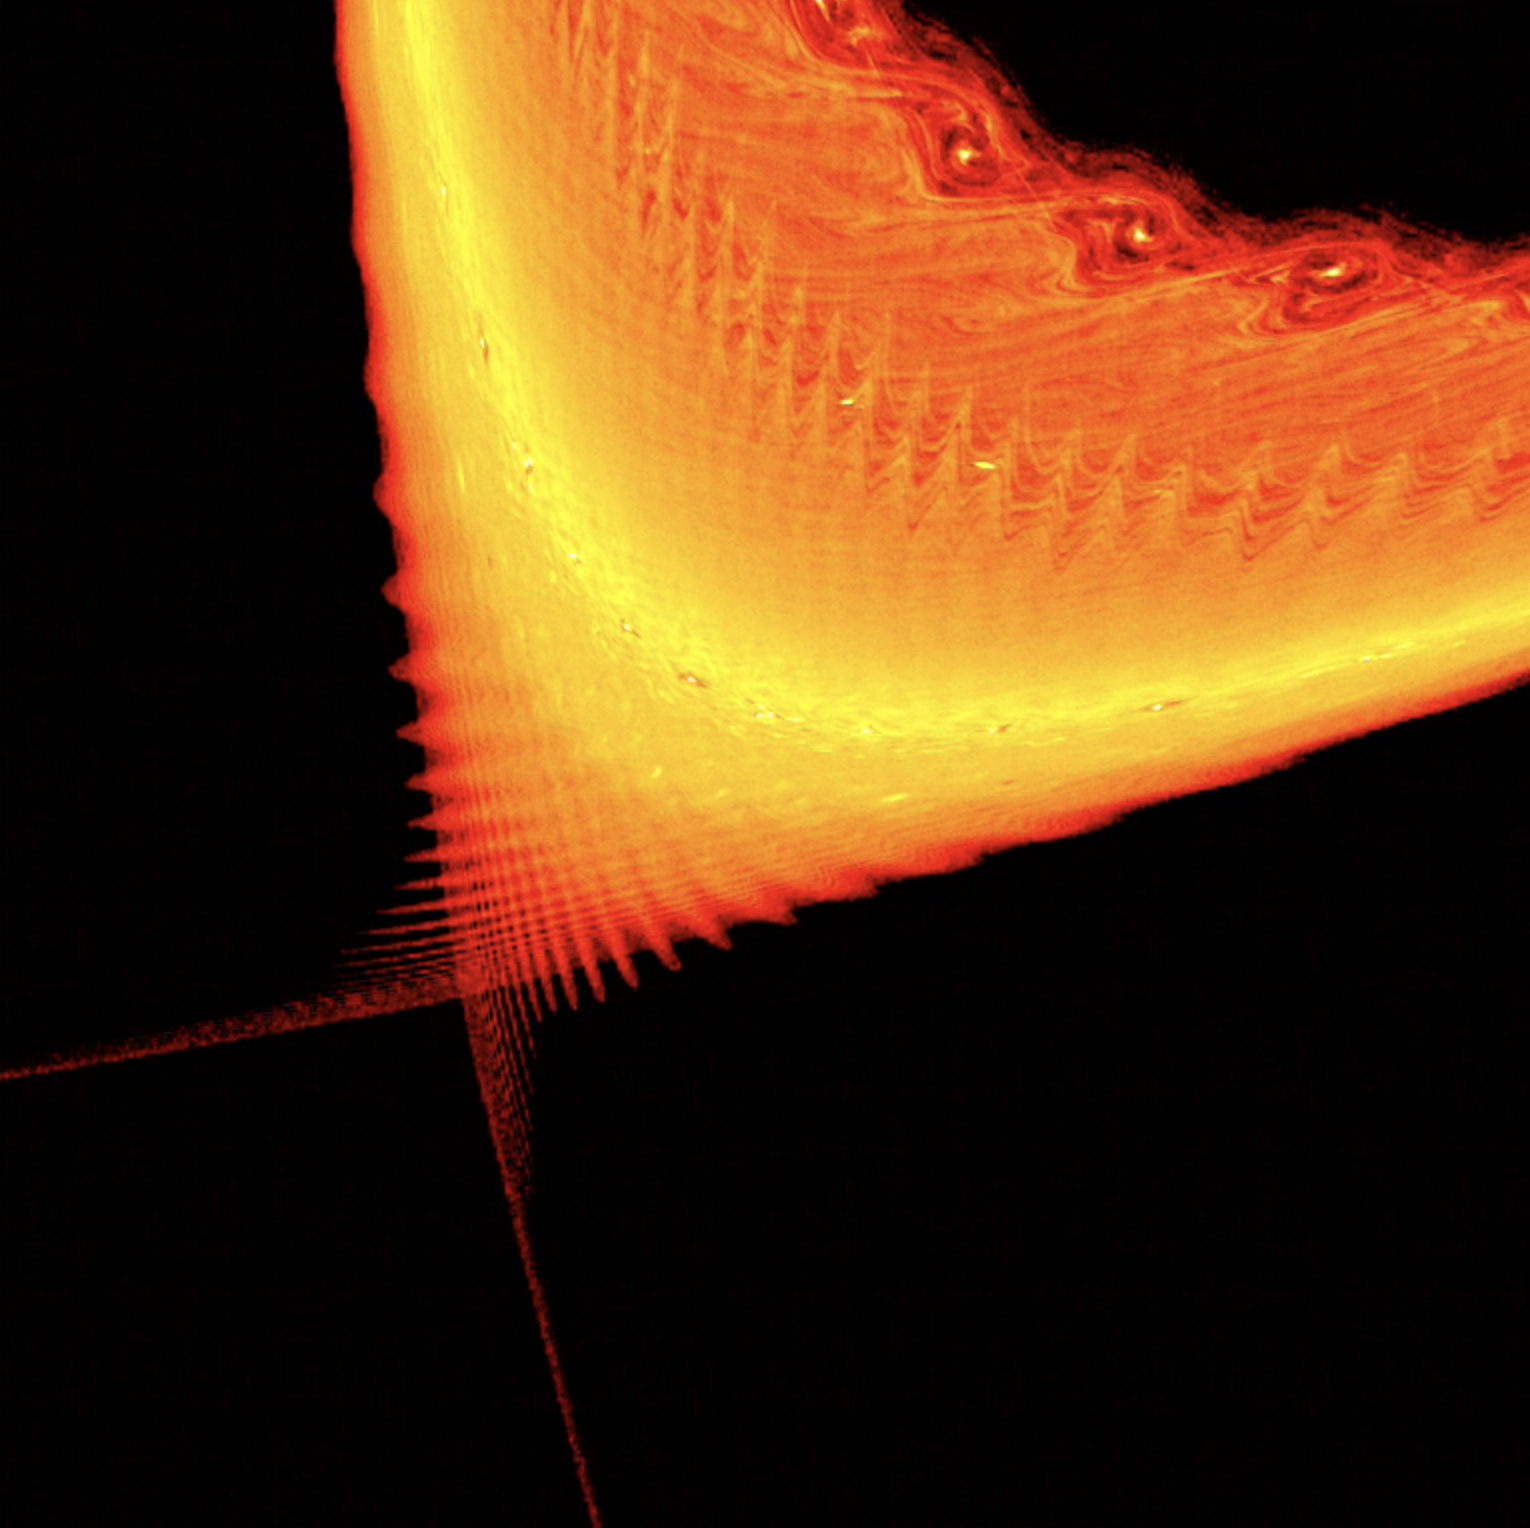
\includegraphics[width=40mm]{figures/poincare-X.2.png}

\caption{\poincare maps generated from two time steps using edge seeding. Zooming in to regions of interest makes it possible to see topological features that develop as the plasma develops.}
\vspace{-5pt}
\label{fig:result}
\end{figure}








\begin{table}[]
\centering
\caption{Time (in seconds) for XGC and \vtkm runs on CPUs and GPUs for both Whole and Edge seeding with $10,240$ and $25,600$ seeds. The time speedup factors for the \vtkm runs on the CPU and GPU are given in two right-most columns.}
\label{table:timingResults}
\begin{tabular}{ll|c|cc|cc}
\hline
\textbf{Num} & \multicolumn{1}{c|}{} & \textbf{XGC} & \multicolumn{2}{c|}{\textbf{VTK-m Time}} & \multicolumn{2}{c}{\textbf{Speedup}} \\
\textbf{Seeds} & \textbf{Seeding} & \textbf{Time} & \textbf{CPU} & \textbf{GPU} & \textbf{CPU} & \textbf{GPU} \\ \hline \hline
10240 & Whole & 2001.8 & 249.0 & 171.5 & \textbf{8.0} & \textbf{11.7} \\
10240 & Edge & 1762.6 & 197.0 & 154.3 & \textbf{8.9} & \textbf{11.4} \\
25600 & Whole & 3785.8 & 655.5 & 245.7 & \textbf{5.8} & \textbf{15.4} \\
25600 & Edge & 3435.3 & 522.0 & 223.1 & \textbf{6.6} & \textbf{15.4} \\ \hline
\end{tabular}
\end{table}


Table~\ref{table:timingResults} contains the timing results for the XGC tool and \vtkm implementations for each configuration.
We also ran the \vtkm implementations using both the Two-Level and Uniform Bins cell locators, but the performances were similar (within $1.5\%$ of each other). The results we report are using the Uniform Bins cell locator. Because the triangles in the cross-sectional grid are uniformly distributed, the added complexity of the Two-Level grid does not provide any benefit. We performed some tuning on the optimal size of the Uniform Bin acceleration structure and found that a size of 12,000$\times$12,000 generally provided the best results.
The speedups for the \vtkm implementation are significant. Running on the CPU, the \vtkm implementation provides between $5.8\times$ and $8.9\times$ speedup over the XGC implementation. On the GPU, \vtkm achieves between $11.4\times$ and $15.4\times$ speedup over the XGC implementation. 
Speedups on the GPU are limited by two factors. First, the number of threads that can be utilized. The computation is parallelized over the seeds, and the number of seeds commonly used for \poincare maps is not enough to saturate the number of threads available on the GPUs. Second, and much more importantly, the cell-finding operation for unstructured grids is bound by the cost of memory access and \emph{not} computation. As the seeds are traced, they circulate throughout the volume in non-uniform ways. Because the acceleration structure used for cell-finding is too large to be kept in fast GPU memory, there is significant time spent accessing data in slower memory spaces.

%\ken{A reviewer might why we don't have a chart for the data in table 1 and/or table 2.}


Table~\ref{table:costSavings} contains a comparison of the total cost (in node-seconds) for the XGC and \vtkm implementations for each configuration. The XGC tool was run on five nodes of Frontier and so the XGC Cost column in Table~\ref{table:costSavings} is $5\times$ the runtime reported in Table~\ref{table:timingResults}. For the \vtkm implementation, the CPU runs were performed on two nodes of Frontier, and the GPU runs were performed on two GPUs within a single node.  Because of this difference in the number of nodes used, the cost savings for the \vtkm implementation are more pronounced than the speedups. For the CPU runs, the \vtkm implementation running on two nodes, results in cost savings between $14.4\times$ and $22.4\times$. For the GPU runs, the \vtkm implementation results in cost savings between $57.1\times$ and $77.1\times$.  We calculate the cost factor for \vtkm using one node, although it technically uses only half of the node, which results in cost savings between $114.2\times$ and $154.2\times$.

The use of fewer nodes becomes even more important when doing in situ processing. XGC uses the in-transit processing model~\cite{ChildsTerminology, Choi2018} for in situ analysis and visualization tasks. In this model, additional nodes are allocated for analysis and visualization. After the simulation completes a time step, the data are transferred to the additional nodes for asynchronous processing.
For simulations that could run for days or weeks, the use of fewer nodes for analysis and visualization results in even more significant cost savings.




\begin{comment}
\begin{table}[]
\caption{Time (in seconds) for XGC and \vtkm runs using the Two-Level (2L) and Uniform Bins (UB) cell locators. The speedup (SU) over the XGC runs is also given for each cell locator type.}
\label{table:timingResults}
\centering
\begin{tabular}{@{~}r@{~~}crr@{~~}rr@{~~}r@{~}}
  \toprule
      &                              & \multicolumn{1}{c}{XGC}      & \multicolumn{2}{c}{\vtkm 2L}                 & \multicolumn{2}{c}{\vtkm UB} \\
  \multicolumn{1}{c@{~~}}{\# Seeds} &
  \multicolumn{1}{@{~~}c}{Seeding} &
  \multicolumn{1}{c}{Time} &
  \multicolumn{1}{c@{~~}}{Time} &
  \multicolumn{1}{@{~~}c}{SU} &
  \multicolumn{1}{c@{~~}}{Time} &
  \multicolumn{1}{@{~~}c}{SU} \\
  \midrule
10240 & Whole & 2001.83 & 168.45 & \textbf{11.88} & 171.49    & \textbf{11.67}   \\
10240 & Edge    & 1762.64 & 150.71 & \textbf{11.70} & 154.29    & \textbf{11.42}   \\
25600 & Whole & 3785.81 & 258.51 & \textbf{14.64} & 245.66    & \textbf{15.41}   \\
25600 & Edge    & 3435.26 & 229.30 & \textbf{14.98} & 223.08    & \textbf{15.40}   \\
  \bottomrule
\end{tabular}
\end{table}
\end{comment}

\begin{table}[]
\centering
\caption{Total cost (in node-seconds) for XGC and the savings factor for the \vtkm runs on the CPU and GPU.
The XGC runs used five nodes and the \vtkm used two Frontier nodes for the CPU runs and one node for the GPU runs.
%\textcolor{red}{Jay: should the metric here be core-time and the unit is node-seconds?} and savings factor for \vtkm.
}
\label{table:costSavings}
\begin{tabular}{ll|r|rr}
\hline
\textbf{Num} & \multicolumn{1}{c|}{} & \multicolumn{1}{c|}{\textbf{XGC}} & \multicolumn{2}{c}{\textbf{VTK-m Cost Savings}} \\
\textbf{Seeds} & \textbf{Seeding} & \multicolumn{1}{c|}{\textbf{Cost}} & \textbf{CPU} & \textbf{GPU} \\ \hline \hline
10240 & Whole & 10009.2 & \textbf{20.1} & \textbf{58.4} \\
10240 & Edge & 8813.2 & \textbf{22.4} & \textbf{57.1} \\
25600 & Whole & 18929.1 & \textbf{14.4} & \textbf{77.1} \\
25600 & Edge & 17176.3 & \textbf{16.5} & \textbf{77.0} \\ \hline
\end{tabular}
\end{table}


\begin{comment}
\begin{table}[]
\caption{Total cost (in node-seconds) for XGC and the savings factor (Factor) for the \vtkm runs using both cell locators.
The XGC runs used five nodes and the \vtkm runs used one Frontier node.
%\textcolor{red}{Jay: should the metric here be core-time and the unit is node-seconds?} and savings factor for \vtkm.
}
\label{table:costSavings}
\centering
\begin{tabular}{r@{~~}crrr}
\toprule
\multicolumn{1}{l}{}          &                              & \multicolumn{1}{c}{XGC}           & \multicolumn{1}{c}{\vtkm 2L} & \multicolumn{1}{c}{\vtkm UB} \\
\multicolumn{1}{c@{~~}}{\# Seeds} & \multicolumn{1}{@{~~}c}{Seeding} & \multicolumn{1}{c}{Cost} & \multicolumn{1}{c}{Factor}   & \multicolumn{1}{c}{Factor}   \\ 
\midrule
10240 & Whole & 10009.15 & 59.42 & 58.37 \\
10240 & Edge    & 8813.20   & 58.48 & 57.12 \\
25600 & Whole & 18929.05 & 73.22 & 77.05 \\
25600 & Edge    & 17176.30  & 74.91 & 77.00 \\
\bottomrule
\end{tabular}
\end{table}
\end{comment}








\begin{comment}
Results on frontier. Kokkos setting:
1000x10 pts, 10 puncs, UB 12000 12000

Setting hints from none, 2 to 1024
0: PoincareTime= 4.59509239
2: PoincareTime= 8.996044041
4: PoincareTime= 5.383845941
8: PoincareTime= 3.334134504
16: PoincareTime= 2.443431037
32: PoincareTime= 1.830533336
64: PoincareTime= 2.019787151
128: PoincareTime= 2.086194197
256: PoincareTime= 2.109982273
512: PoincareTime= 4.521679962
1024: PoincareTime= 6.577413594

1000x10 pts, 100 puncs
0: PoincareTime= 44.886269575
2: PoincareTime= 86.530851057
4: PoincareTime= 53.34156569
8: PoincareTime= 31.379374444
16: PoincareTime= 22.082198616
32: PoincareTime= 15.638019499
64: PoincareTime= 18.477414351
128: PoincareTime= 18.550843151
256: PoincareTime= 20.639840234
512: PoincareTime= 45.01590981
1024: PoincareTime= 76.879381214

Hints=32
whole:
10k x 1000: 149.154060158
25k x 1000:  309.024710581
edge: 
10k x 1000: 140.758010554
25k x 1000: 


whole: 10k x 1000
Hints-32  149.154060158
Hints=64  180.872969537
Hints=128  187.471073264

whole: 25k x 1000
Hints=32 309.024710581
Hints=64 267.215708676
Hints=128 267.135570261


Vary UB:
10k x 10punc
12: 1.811252
10: 1.665629376
8: 1.548936766
4:  1.443947304
2: 1.527570323
but at 100 puncs, 10k 12k is best.


10k x 1000punc, UB12
Whole
H32: 147.828542898
H64: 182.412161965
H128: 187.174267512

Edge
H32: 139.308568648
H64: 154.220764795
H128: 155.587906359

25k x 1000punc, UB12
Whole
H32: 309.551289458
H64: 269.644134008
H128: 267.333313573

Edge
H32: 290.064207587
H64: 223.823065319
H128: 221.518910766



2L:
8 2 1.422736871
16 2 1.398853571
32 2 1.972269867
64 2 2.044388573
128 2 2.075921773


openmp

\end{comment}
